\clearpage
\begin{flushright}
	\textit{Лекция №19}
	\textit{2015.11.24}
\end{flushright}

В тупик попадают взаимодействующие процессы.

2. Упорядочиваем ресурсы. Ресурсы делятся на классы. Каждому такому классу присваивается номер и выполняется следующее правило: процессы могут запрашивать ресурсы из классов с номерами большими, чем номера классов, к которым принадлежат классы, которые уже удерживают. Если он запрашивает ресурс с номером меньше, чем те, которые он уже удерживает, то он должен освободить все, что удерживает и запросить всё заново. Так он вырождается в первый способ (ему нужно всё опять запросить разом).

3. У процессов можно отбирать ресурсы, устраняет свойство неперераспределимости ресурсов. Если процесс, в процессе запроса, не может получить ресурс, то он должен освободить уже занятые ресурсы. Этот подход может привести к запросу и освобождению одних и тех же ресурсов (трешинг).

\paragraph{Обход тупиков}. Единственным классическим подходом к обходу тупиков является алгоритм банкира, предложенный Дейкстрой. Банкиры дают заём. Задача банкира – дать заём тем, кто может их вернуть, но часто заемщик не может вернуть заем сразу, да и то, ему нужны еще заёмы. Банкир – менеджер системы. Заемы – процессы, делающие заявки на ресурсы, заявка процесса должна отображать максимальную потребность в ресурсе каждого класса. В процессе выполнения, процесс не может затребовать ресурсов больше, чем указал в заявке. Кол-во процессов – фиксировано. В системе должна быть информация, для этого определяются специальные структуры, при этом процесс запрашивает ресурсы по единице. МР гарантирует, что в системе тупик не возникнет. Каждый запрос проверяется по отношению к кол-ву ресурсов данного типа, имеющихся в системе. Анализируя ситуацию, МР ищет такую последовательность процессов, которая с учетом максимальных потребностей в ресурсе данного типа может завершиться. Если такая последовательность есть, то система не находится в тупике и состояние системы надежно, в результате запрошенные единицы ресурса выделяется процессу.

\begin{table}[H]
\caption{Надежное состояние}
\label{tbl:norm_state}
\begin{tabular}{|l|l|l|l|}
\hline
процессы & текущее распределение & свободные единицы & заявка \\
\hline
p1 & 1 &  & 4\\
\hline
p2 & 3 &  & 5\\
\hline
p3 & 5 &  & 9\\
\hline
 &  & 2 & \\
 \hline
\end{tabular}
\end{table}

\ref{tbl:norm_state} является надежной и безопасной относительно тупика, так как в таблице имеется последовательность процессов, которая может завершиться. 
Если текущее состояние системы надежно, то все последующие состояния системы будут надежными. Например, если система из состояния в \ref{tbl:norm_state}  перейдет в следующее состояние \ref{tbl:no_norm_state}

\begin{table}[H]
\caption{Надежное состояние}
\label{tbl:norm_state}
\begin{tabular}{|l|l|l|l|}
\hline
процессы & текущее распределение & свободные единицы & заявка \\
\hline
p1 & 2 &  & 4\\
\hline
p2 & 3 &  & 5\\
\hline
p3 & 5 &  & 9\\
\hline
 &  & 1 & \\
 \hline
\end{tabular}
\end{table}

В такой ситуации нет последовательности.  Но процессы могут и не запросить максимально заявленное кол-во ресурсов. Состояние системы является безопасным, если существует последовательность процессов такая, что первый процесс в последовательности обязательно завершится, так как если он запросит максимально заявленное кол-во ресурсов, то в системе хватит ресурсов. Второй процесс может завершиться, если первый процесс завершится и вернет занимаемые им ресурсы, и в сумме этих ресурсов будет достаточно для удовлетворения потребностей. И так далее. 
Когда процесс делает новый запрос, менеджер ресурсов должен найти последовательность успешно завершаемых процессов, и только в этом случае запрос будет удовлетворен.  Запрос процесса, переводящий систему в ненадежное состояние – откладывается. Так как система постоянно поддерживается в надежном состоянии, то за конечное время все запросы будут завершены и все процессы смогут завершить свою работу, но каждый раз требуется исследовать n! последовательностей, что предполагает большие затраты на выполнение данного алгоритма. Таким образом, алгоритма банкира имеет теоретическое значение.
Это важно для систем реального времени, которые управляют внешними по отношению к системе процессами. Чаще всего это системы автопилота, ставятся в автомобили. Не нужно путать систему реального времени с системой разделения времени. 

Предлагаются подходы аппроксимации алгоритма банкира. Наиболее известная, это \paragraph{алгоритм Габермана}. МР поддерживает массив:\\
$S[0..r-1]$ //$r$ - число единиц ресурса\\
$S[i] = r - 1$ для всех $i: 0 <= i <= r$\\
заявил - С, удерживает - H, и запрашивает 1, то $S[i]$ декрементируется для всех $i: 0 <= i <= C - H$.  Если какое то из $S[i]$ становится отрицательным, то такое состояние системы становится опасным, относительно тупика.
Затратность этого алгоритма значительно меньше, чем $N^2$. 


\paragraph{Третий способ обнаружения тупиков}: опасная цепь запросов обнаруживается с помощью графов. Для обнаружения тупиков используется модель Хомта, представляет собой двудольный (бихроматический) граф, разбивается на два подмножества, множество вершин процессов, множество вершин ресурсов. Вершины соединяются дугами, причем одна дуга не соединяет вершины одного и того же множества. Граф направленный. Дуга, которая выходит из вершины подмножества вершин ресурсов к вершине из подмножества вершин процессов, называется выделением ресурса. И дуга, которая выходит из вершины процесса и входит в вершину ресурса называется запросом. Тупики обнаруживаются методом редукции графа. Редукция заключается в ??? дуг графа. Если все вершины становятся изолированными, то система не находится в тупике.

\begin{figure}[H]
    \centering
    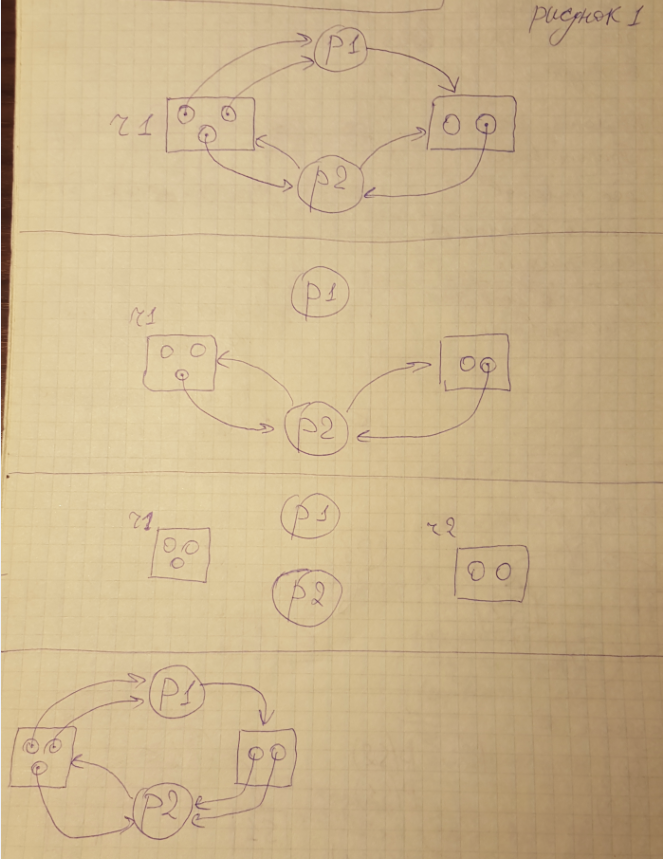
\includegraphics[width=\textwidth]{pic/1.png}
    \caption{pic}
    \label{pic:graph_tupik}
\end{figure}

Данный граф \ref{pic:graph_tupik} можно сократить по вершине $Р1$, так эта вершина становится изолированной.

Шоу было доказано ряд теорем:
\begin{enumerate}
    \item Граф является полностью сокращаемым, если существует такая последовательность сокращения, которая устраняет все дуги. Если граф нельзя полностью сократить, то анализируемое состояние является тупиковым. 
    \item Цикл, в графе повторно используемых ресурсов, является необходимым условием тупика.
    \item Если состояние $S$ не является состоянием тупика, то состояние $T$, в которое система переходит из $S$ и $T$ есть состояние тупика, то в ??? когда операция процесса $P_i$ является запросом. $P_i$  находится в тупике в состоянии $T$. Т.е. тупик в системе может возникнуть только в результате запроса.     
\end{enumerate} 

\begin{figure}[H]
    \centering
    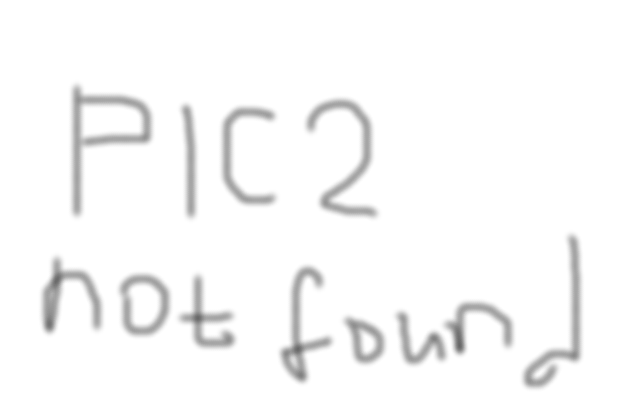
\includegraphics[width=\textwidth]{pic/2.png}
    \caption{демонстрирует несокращаемый граф}
\end{figure}

Представление графов в системе: двудольный бихроматический граф может быть представлен двумя матрицами, матрицей запросов $A{p, r}$ ($a_{ij}$ – запрос $i$ процесса на единицу $j$ ресурса) и матрицей распределения $B{r, p}$ ($b_{ij}$ – кол-во единиц $i$ ресурса выделенное $j$ процессу). Можно также делать связный список. Очевидно, что и матрицы, и списки должны быть монопольно используемыми, это представление двудольного графа.

Алгоритмы обнаружения:\\
1. Метод прямого обнаружения заключается в просмотре по порядку матрицы и там где это возможно производится сокращение, действия аналогичные сокращению дуг графа, до тех пор, пока нельзя будет сделать еще сокращений. Процессы, оставшиеся после всех сокращения, находятся в тупике. Для самого плохого случая, когда сокращения выполняются в порядке, обратном следованию процессов, число проверок будет $n * (n + 1) /2$. Каждая проверка требует просмотра $N$  ресурсов, таким образом время для выполнения данных действий будет пропорционально  $m * n^2$\\
2. Алгоритм с вектором свободных ресурсов$ F = [..f_j]$, где $f_j$ – кол-во свободных единиц ресурсов. Тогда кол-во распределенных единиц $j$ ресурсов, и кол-во свободных единиц $j$ ресурса равно кол-ву единиц этого ресурса в системе. $$r_j = f_j + \sum\limits_{j} b_{ji}$$
Основан на анализе запросов путем сравнения векторов. Пусть имеется два вектора $C$ и $D$. $C <= D : ci <= di$ для $1 <= i <= n$ . Когда ??? и строка запросов этого процесса меньше или равна вектора $F$ то такой запрос может быть удовлетворен.